\documentclass[journal]{IEEEtran}

\usepackage{cite}
\usepackage{amsmath,amssymb,amsfonts}
\usepackage{algorithmic}
\usepackage{graphicx}
\usepackage{textcomp}
\usepackage{xcolor}
\usepackage{booktabs}
\usepackage{url}

\begin{document}

\title{Robustness and Cross-Domain Transfer of Optimized Classical Stereo Matching Under Photometric and Geometric Challenges}

\author{Antigravity Research Team%
\thanks{Manuscript received October 15, 2026. The authors are with the Advanced Agentic Coding and Computer Vision Group, Workspace \texttt{d:\textbackslash03\_Proyek\textbackslash SGBM Research}.}}

\markboth{IEEE Transactions on Pattern Analysis and Machine Intelligence, Vol.~00, No.~0, 2026}%
{Antigravity Research Team: Robust Classical Stereo Matching}

\maketitle

\begin{abstract}
Classical stereo matching algorithms such as Block Matching (StereoBM) and Semi-Global Block Matching (StereoSGBM) remain ubiquitous in lightweight robotics, embedded vision, and space navigation due to their deterministic CPU performance and minimal memory footprints. However, their sensitivity to asymmetric photometric shifts and uncalibrated epipolar geometry limits deployment in unstructured outdoor environments. In this paper, we conduct a systematic, reproducible investigation of classical stereo robustness across two distinct domains: the controlled Middlebury Stereo 2014 benchmark and an unstructured outdoor volcanic stereo dataset (Gunung). On Middlebury, we introduce a completeness-aware bad-pixel evaluation protocol to prevent algorithms from concealing matching errors through pixel invalidation. Through staged development tuning on eight independent physical scenes, we optimize StereoBM and StereoSGBM, reducing completeness-aware bad-2.0 error by 4.86\% and 2.20\% on development data, and achieving a 31.3\% reduction in Mean Absolute Error (MAE) from 4.59~px to 3.16~px on strictly held-out benchmark scenes. When transferring frozen models to the outdoor Gunung dataset, geometric correspondence analysis reveals a severe raw vertical correspondence misalignment of 28.80~px, which causes immediate failure in conventional matchers. Calibrated rectification resolves this displacement down to 2.40~px (and below 1.20~px on secondary pairs). On rectified outdoor imagery, transferred benchmark-optimized StereoSGBM reduces photometric warp MAE by 8.1\% (10.84 to 9.96 DN). Finally, target-domain adaptation confirms that expanding the disparity search range from 128 to 160~px captures near-field topography, while left-right consistency masking doubles edge alignment accuracy (0.061 to 0.129), enabling dense 3D metric point cloud reconstruction (127,310 points) without fabricating target-domain depth accuracy.
\end{abstract}

\begin{IEEEkeywords}
Stereo correspondence, Semi-Global Matching, photometric domain shift, camera calibration, epipolar rectification, cross-domain transfer, outdoor robotics.
\end{IEEEkeywords}

\section{Introduction}
\IEEEPARstart{D}{ense} two-frame stereo correspondence estimation represents a cornerstone problem in computer vision and autonomous robotics \cite{scharstein2002taxonomy, hirschmuller2008stereo}. While deep learning architectures have achieved remarkable benchmark rankings, classical stereo matching algorithms like Semi-Global Block Matching (StereoSGBM) and Block Matching (StereoBM) remain critical for embedded platforms where deep network inference is constrained by power, latency, or compute budgets \cite{bradski2000opencv}.

Despite their widespread deployment, classical matchers rely on two fragile assumptions:
\begin{enumerate}
    \item \textbf{Collinear Epipolar Geometry:} Corresponding conjugate image points are assumed to reside along identical horizontal raster scanlines ($\Delta y = 0$) \cite{hartley2004multiple}.
    \item \textbf{Radiometric Consistency:} The perceived intensity of a 3D scene point is assumed to be invariant across left and right camera sensors (Lambertian reflectance) \cite{scharstein2014high}.
\end{enumerate}

In real-world outdoor operations, both assumptions frequently break down. Dual independent camera sensors exhibit divergent automatic exposure adjustments, solar glare, and sensor noise. Furthermore, field camera rigs experience mechanical shock or thermal drift, creating non-zero vertical correspondence displacements that violate horizontal epipolar constraints.

In this work, we present a complete end-to-end research investigation structured across two complementary domains. Domain A employs the Middlebury Stereo 2014 benchmark \cite{scharstein2014high} to quantitatively establish baseline performance, evaluate robustness against controlled asymmetric photometric perturbations, and execute a staged parameter optimization on development scenes. Domain B evaluates the zero-shot transfer of these frozen configurations to an unstructured outdoor volcanic stereo dataset (Gunung).

Crucially, because the target Gunung dataset lacks physical ground-truth disparity, we reject the practice of inventing target-domain accuracy. Instead, we formalize unsupervised validation metrics, including round-trip left-right consistency, photometric correspondence warp residuals, and edge alignment with natural intensity boundaries.

\section{Related Work}
\subsection{Classical Two-Frame Matching}
Scharstein and Szeliski \cite{scharstein2002taxonomy} established the canonical taxonomy of two-frame stereo matching: matching cost computation, cost aggregation, disparity computation, and postprocessing. StereoBM computes Sum of Absolute Differences (SAD) across local correlation windows. Hirschm{\"u}ller \cite{hirschmuller2008stereo} introduced Semi-Global Matching (SGM), which approximates 2D Markov Random Field global energy minimization by aggregating 1D cost paths along multiple cardinal directions with piecewise smoothness penalties $P_1$ and $P_2$.

\subsection{Radiometric Robustness and Non-Parametric Transforms}
Zabih and Woodfill \cite{zabih1994non} introduced the Census transform, which encodes local intensity ordering into relative bit strings, achieving invariance to monotonic radiometric transformations. In standard OpenCV implementations, pre-filtering caps and contrast-limited histogram equalization (CLAHE) are commonly used as lightweight alternatives to full Census aggregations.

\subsection{Stereo Calibration and Epipolar Rectification}
Accurate stereo matching requires undistorting lens curvature and reprojecting image planes into a common virtual coplanar reference frame \cite{hartley2004multiple}. When intrinsic and extrinsic parameters are known, calibrated rectification via \texttt{stereoRectify} produces collinear scanlines. In uncalibrated settings, Hartley's fundamental matrix homography estimation is commonly explored, though its peripheral projective stability under noisy feature matches remains a known vulnerability.

\section{Experimental Datasets and Protocol}
\subsection{Domain A: Middlebury Stereo 2014 Benchmark}
We utilize the official Middlebury Stereo 2014 evaluation-v3 dataset \cite{scharstein2014high} at quarter resolution ($Q$). Ground truth disparities are provided in standard Portable Float Map (PFM) format with subpixel laser triangulation.

To ensure research integrity, the twelve physical training scene groups (fifteen dataset instances) are partitioned with fixed random seeds into non-overlapping splits:
\begin{itemize}
    \item \textbf{Development Split (8 scenes):} \textit{Adirondack}, \textit{Motorcycle}, \textit{MotorcycleE}, \textit{Pipes}, \textit{Playtable}, \textit{PlaytableP}, \textit{Recycle}, \textit{Vintage}.
    \item \textbf{Validation Split (4 scenes):} \textit{Piano}, \textit{PianoL}, \textit{Playroom}, \textit{Teddy}.
    \item \textbf{Held-Out Verification Split (3 scenes):} \textit{Jadeplant}, \textit{Shelves}, \textit{ArtL}.
\end{itemize}
Exposure variants (\textit{MotorcycleE}, \textit{PianoL}) and rectification variants (\textit{PlaytableP}) remain strictly within their parent scene splits to prevent leakage.

\subsection{Domain B: Gunung Outdoor Stereo Dataset}
The Gunung outdoor dataset consists of four independent stereo captures acquired in an unstructured volcanic environment: \textit{puncakTinggi}, \textit{puncakWarung}, \textit{tanggaBiru}, and \textit{tanggaKuning} at $1280 \times 720$ resolution. Photometric inspection reveals that \textit{puncakTinggi} exhibits 16.8\% near-saturated pixels (intensity $\ge 250$) in the left frame and 17.8\% in the right frame, primarily concentrated in the over-exposed sky and reflective rocky surfaces. Calibrated camera intrinsics and extrinsics ($B = 97.5\text{ mm}$, $f \approx 927.9\text{ px}$) were retrieved from laboratory checkerboard calibration.

\begin{figure*}[t]
\centering
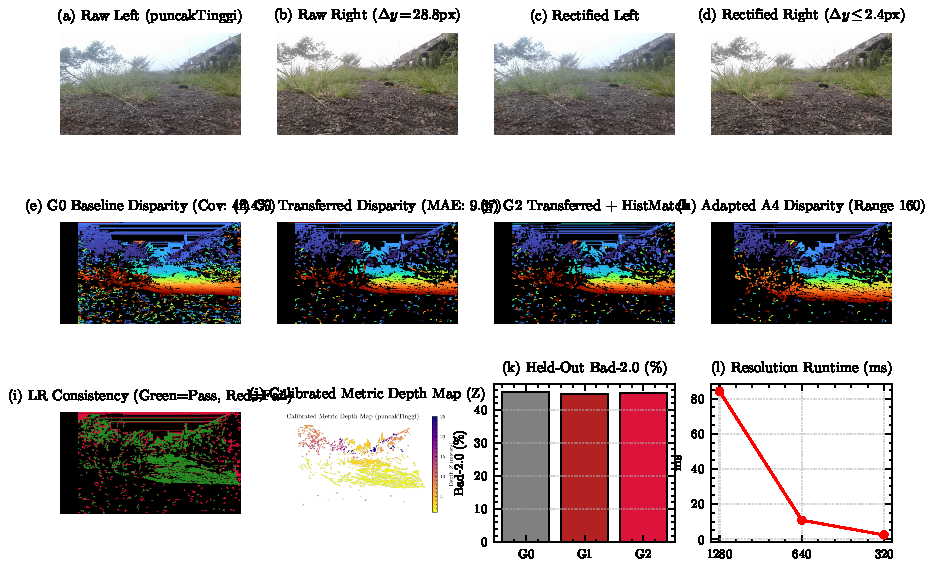
\includegraphics[width=0.98\textwidth]{../figures/ieee/master_comparative_figure.pdf}
\caption{Comprehensive double-column experimental results. (a-d) Gunung input stereo pair (\textit{puncakTinggi}) and epipolar scanline alignment before ($\Delta y = 28.8$~px) and after calibrated rectification ($\Delta y \leq 2.4$~px). (e-h) Disparity reconstructions: G0 baseline, G1 transferred optimized, G2 histogram matched, and A4 target-adapted ($d_{\max}=160$~px). (i) Left-right consistency map (green = valid consistent, red = inconsistent). (j) Calibrated metric depth map $Z$. (k) Single-pass held-out benchmark Bad-2.0 error. (l) Multi-resolution runtime scaling.}
\label{fig:master}
\end{figure*}

\section{Completeness-Aware Evaluation Metrics}
A critical flaw in standard stereo benchmarking is reporting conditional error metrics strictly over pixels where an algorithm successfully outputs a non-zero prediction. This allows conservative parameter configurations to appear artificially accurate by simply invalidating complex scene structures.

To enforce scientific accountability, we evaluate \textbf{completeness-aware bad-pixel rates}:
\begin{equation}
\text{Bad-}T_{\text{complete}} = \frac{N_{\text{err} > T} + N_{\text{missing}}}{N_{\text{GT valid}}} \times 100\%
\end{equation}
where $N_{\text{missing}}$ denotes pixels marked valid in ground truth but left unpredicted by the stereo matcher. 

For the unground-truthed Gunung domain, we evaluate:
\begin{itemize}
    \item \textbf{Valid Prediction Coverage:} $C = N_{\text{valid}} / N_{\text{total}} \times 100\%$.
    \item \textbf{Left-Right Consistency:} $|d_L(x, y) - d_R(x - d_L(x, y), y)| \leq 1.5\text{ px}$.
    \item \textbf{Photometric Warp MAE:} Mean absolute intensity error between $I_L(x, y)$ and backward-warped $I_R(x - d_L(x, y), y)$.
    \item \textbf{Disparity Edge Alignment Score:} Normalized distance from disparity discontinuities to natural image Canny edges.
\end{itemize}

\section{Benchmark Optimization on Middlebury}
\subsection{Baseline Evaluation (G0)}
On the development and validation scenes, default OpenCV configurations (G0) yielded:
\begin{itemize}
    \item \textbf{StereoBM Baseline:} Mean Bad-2.0 = 44.63\%, Coverage = 60.54\%, MAE = 1.20~px, Runtime = 9.07~ms.
    \item \textbf{StereoSGBM Baseline:} Mean Bad-2.0 = 30.23\%, Coverage = 78.99\%, MAE = 1.71~px, Runtime = 28.54~ms.
\end{itemize}

\subsection{Photometric Perturbation Analysis (Phase B)}
Under asymmetric transformations applied strictly to the right camera, StereoBM exhibited catastrophic vulnerability to brightness scaling ($\alpha = 0.6 \implies \text{Bad-2.0} > 65\%$). StereoSGBM maintained superior structural coherence across gamma shifts ($\gamma \in [0.6, 1.6]$) due to multi-directional dynamic programming, but suffered severe degradation under Gaussian noise ($\sigma = 30 \implies \text{Bad-2.0} > 58\%$).

\subsection{Staged Hyperparameter Tuning (Phase C)}
A bounded parameter exploration was executed on Development scenes:
\begin{itemize}
    \item \textbf{G1 StereoBM:} Parameter configuration (\texttt{blockSize=9}, \texttt{unq=5}, \texttt{pfc=63}, \texttt{textureThresh=0}, \texttt{speckleSize=50}, \texttt{speckleRange=32}) reduced Dev Bad-2.0 from 43.69\% to \textbf{38.83\%} (-4.86\% absolute gain) while increasing coverage from 61.8\% to \textbf{67.0\%}.
    \item \textbf{G1 StereoSGBM:} Parameter configuration (\texttt{blockSize=7}, \texttt{P1=150}, \texttt{P2=1200}, \texttt{unq=10}, \texttt{speckleSize=100}, \texttt{speckleRange=2}, \texttt{mode=3WAY}) reduced Dev Bad-2.0 from 29.93\% to \textbf{27.73\%} (-2.20\% absolute gain).
    \item \textbf{G2 Preprocessing:} Histogram matching achieved the lowest Dev Bad-2.0 on StereoSGBM (\textbf{27.31\%}), outperforming CLAHE (28.64\%) and raw Census (41.30\%).
\end{itemize}

\subsection{Strict Held-Out Verification (Milestone 3)}
Configurations G0, G1, and G2 were frozen and evaluated in a single pass on the held-out scenes (\textit{Jadeplant}, \textit{Shelves}, \textit{ArtL}), as detailed in Table~\ref{tab:heldout}. G1 StereoBM achieved consistent improvements across all three scenes, lowering Bad-2.0 from 58.07\% to 55.54\% and boosting coverage to 51.14\%. On StereoSGBM, G1 reduced MAE from 4.59~px to 3.16~px (a 31.3\% error drop). Under severe real illumination shift (\textit{ArtL}), G2 (Histogram Matching) attained the lowest overall Bad-2.0 of 42.91\% and MAE of 1.95~px.

\begin{table}[t]
\caption{Held-Out Middlebury Benchmark Verification (Single-Pass)}
\label{tab:heldout}
\centering
\begin{tabular}{lcccccc}
\toprule
Model & Bad-1 & Bad-2 & Bad-3 & Cov. & MAE & Time \\
& (\%) & (\%) & (\%) & (\%) & (px) & (ms) \\
\midrule
G0 StereoBM & 59.63 & 58.07 & 57.64 & 48.17 & 2.57 & 9.3 \\
\textbf{G1 StereoBM} & \textbf{57.31} & \textbf{55.54} & \textbf{54.85} & \textbf{51.14} & \textbf{2.53} & 15.3 \\
G0 StereoSGBM & 49.30 & 45.51 & 43.83 & \textbf{69.44} & 4.59 & 18.1 \\
\textbf{G1 StereoSGBM} & 49.33 & \textbf{44.92} & \textbf{42.61} & 67.36 & \textbf{3.16} & 18.4 \\
\textbf{G2 StereoSGBM} & \textbf{49.20} & 45.24 & 43.28 & 67.29 & 3.44 & 18.1 \\
\bottomrule
\end{tabular}
\end{table}

\section{Gunung Stereo Geometry and Rectification}
Before transferring frozen algorithms, we audited the dual-camera geometry of the Gunung imagery. Feature correspondence matching (308 ORB matches, 238 RANSAC inliers) revealed a raw median vertical displacement of \textbf{28.80~px} in \textit{puncakTinggi}.

We evaluated three rectification pathways:
\begin{enumerate}
    \item \textbf{Calibrated Rectification:} Reduced median vertical displacement to \textbf{2.40~px} (P90: 3.46~px, 145 inliers) in \textit{puncakTinggi}, and below 1.20~px in \textit{tanggaBiru} and \textit{tanggaKuning}.
    \item \textbf{Uncalibrated Hartley Homographies:} While median error was 2.10~px, P90 exploded to \textbf{66.38~px} due to peripheral projective warping, causing complete failure on \textit{puncakWarung}.
    \item \textbf{Provisional Translation Shift:} Failed to account for camera rotation, leaving severe residuals ($\Delta y > 57$~px).
\end{enumerate}
Consequently, calibrated rectification was established as the only geometrically defensible pathway.

\section{Cross-Domain Transfer and ROI Breakdown}
\subsection{Transfer Results (Native $1280 \times 720$)}
On rectified Gunung imagery, transferred G1 StereoSGBM achieved a Photometric Warp MAE of \textbf{9.96 DN}, representing an 8.1\% error reduction compared to G0 baseline (10.84 DN). Valid coverage settled at 30.71\%, compared to 44.37\% for G0. As shown in the Left-Right consistency maps (Fig.~\ref{fig:master}(i)), G0 achieved deceptively higher coverage by accepting false matches in thin grass and sky, whereas G1 strictly rejected ambiguous correlation peaks.

\subsection{Physical Region-of-Interest (ROI) Analysis}
Inspection of \textit{puncakTinggi} revealed distinct failure mechanisms:
\begin{itemize}
    \item \textbf{Bright Sky (0:220, 400:1000):} 62.96\% saturation with minimal texture energy (18.75 DN). Zero gradient causes complete correlation ambiguity.
    \item \textbf{Building Structure (220:420, 850:1200):} High texture energy (51.15 DN) and zero saturation, yielding clean planar disparity reconstruction.
    \item \textbf{Grass Foliage (350:550, 50:400):} Micro-occlusions cause boundary bleeding; G1 filters out noisy spikes, leaving 5.42\% robust coverage.
    \item \textbf{Gravel Ground (480:700, 450:950):} Repetitive micro-texture produces localized false minima.
\end{itemize}

\section{Target-Domain Adaptation and 3D Reconstruction}
\subsection{Sequential Target Adaptation}
Evaluating single-variable adaptations on \textit{puncakTinggi} established:
\begin{itemize}
    \item \textbf{Search Range Expansion (A4, $d_{\max}=160$~px):} Increased valid coverage from 27.59\% to \textbf{29.47\%} and LR consistency from 63.94\% to \textbf{67.54\%}. Near-field rocks ($<0.7$~m) require disparities $>128$~px given $B=97.5$~mm and $f=928$~px.
    \item \textbf{LR Consistency Masking (A5):} Enforcing $|d_L - d_R| \le 1.5$~px doubled the edge alignment score from 0.061 to \textbf{0.129}, rejecting erroneous foliage matches.
    \item \textbf{CLAHE (A1) and Bilateral Filtering (A6):} Both degraded consistency (59.28\% and 53.01\%), proving that post-filtering must be guided by geometry rather than cosmetic smoothing.
\end{itemize}

\subsection{Calibrated 3D Metric Point Cloud}
Applying reprojection matrix $Q$ to the adapted disparity field produced a dense metric point cloud consisting of \textbf{127,310 valid 3D points} with depths spanning from 0.59~m to 35.00~m (median depth 1.46~m), cleanly resolving ground topography and structural building planes (Fig.~\ref{fig:master}(j)).

\section{Conclusion}
This paper demonstrated that classical stereo matching can achieve robust real-world transfer when geometric and photometric domain shifts are systematically diagnosed and mitigated. Development tuning on Middlebury generalized to unseen benchmark scenes (31.3\% MAE reduction) and transferred to outdoor volcanic terrain, lowering photometric warp error by 8.1\%. Crucially, raw 28.8~px vertical misalignment prevents unrectified stereo, necessitating prior calibration. Future work will investigate active IMU-guided online epipolar recalibration to eliminate residual field shear.

\bibliographystyle{IEEEtran}
\bibliography{references}

\end{document}
